\section{Evaluation}
\label{sec:evaluation}

All figures in this section are on the evaluation draw's test period (\nTestRows{} rows holding
\nTestFraud{} confirmed fraud), for models trained on \nTrainUsed{} rows holding
\nGateTrainFraud{} confirmed fraud.

\subsection{Gate metrics as margins over the floor}

Table~\ref{tab:gate} reports each ranking metric beside the best single feature and the best
trivial rule on the same rows. On these rows the best single feature, again
\texttt{velocity\_ratio\_1h\_vs\_30d}, reaches \nGateFloor{}; the ensemble's margin over it is
\nGateMargin{}. The narrowest margin is USSD's, \nGateUSSDMargin{}, the channel with no device
fingerprint.

\begin{table}[htbp]
\centering
\caption{Ranking metrics of the calibrated ensemble, with the best single feature
(\texttt{velocity\_ratio\_1h\_vs\_30d}) on the same rows and the margin over it. Draw
\texttt{d8083dbc}, test period of \nTestRows{} rows holding \nTestFraud{} fraud, evidence commit
\texttt{d40fca2}, source \texttt{docs/benchmarks/m4\_gate\_d8083dbc\_v3.txt}.}
\label{tab:gate}
\begin{tabular}{lrrr}
\toprule
Metric & Ensemble & Single feature & Margin \\
\midrule
AUC-ROC & \nGateAUC{} \nGateAUCci & \nGateFloor & \nGateMargin \\
Recall at \nFPRBudget{} FPR & \nGateRecallFPR{} \nGateRecallFPRci & \nGateRecallFPRFloor & \nGateRecallFPRMargin \\
AUC, \texttt{MOBILE\_MONEY} & \nGateMM & \nGateMMFloor & \nGateMMMargin \\
AUC, \texttt{USSD} & \nGateUSSD & \nGateUSSDFloor & \nGateUSSDMargin \\
AUC, \texttt{AGENT\_BANKING} & \nGateAgent & \nGateAgentFloor & \nGateAgentMargin \\
\bottomrule
\end{tabular}
\end{table}

The best trivial rule (one threshold on \texttt{amount\_log1p}) reaches \nGateTrivial{}, a margin
of \nGateTrivialMargin{}. The remaining gate metrics are read at a calibrated probability, which a
lone feature does not have, so no floor exists for them and none is quoted: at the flag threshold
recall is \nGateRecallSix{} \nGateRecallSixci{} against a target of \nTargetRecall{} and the
false-negative rate \nGateFNR{} against \nTargetFNR{}, the two metrics that \textbf{fail}; F1 is
\nGateFone{} \nGateFoneci{}; the false-positive rate at the block threshold is \nGateFPRBlock{};
SHAP coverage of flagged transactions is \nGateShapCov{}; and the expected calibration error over
15 equal-mass bins is \nGateECE{}. In all, \nGatePass{} gate metrics pass.

The recall miss is recorded as a finding at this training volume, with the threshold unchanged and
nothing tuned on the test period (ADR 0031). It is a shortfall in ranking, not a choice of
threshold: even at the looser \nFPRBudget{} false-positive budget recall is \nGateRecallFPR{},
still below \nTargetRecall{}, so no threshold on this run reaches the target. Whether the miss is a
property of the benchmark or of training on \nTrainUsed{} of the \nTrainRows{} available rows is
untested until the learning curve (PB-67) is measured: \notyet{PB-67 learning curve}. At the flag
threshold precision is \nGatePrecSix{}, so the operating point trades recall for very few false
alerts.

Precision at the \nFPRBudget{} budget is \nGatePrecFPR{}, reported against its ceiling at this
test period's base rate, \nGatePrecCeiling{}: even a perfect ranking could not exceed it, which is
why the specification's precision target at this rate was replaced (resolution D-01). Over
\nSeeds{} refits the AUC is \nGateSeedAUC{} and recall at the flag threshold
\nGateSeedRecallSix{}. Export parity: the maximum absolute difference between ONNX and native
scores over the whole test period is \nGateOnnx{}.

\paragraph{What each slice rests on.} Table~\ref{tab:slices} gives the test period by channel and by
country, with the fraud count behind every per-channel and per-country AUC in this paper. The
rows and fraud sum to the test period's \nTestRows{} and \nTestFraud{}. The three channel AUCs of
Table~\ref{tab:gate} are the ensemble's; the others are the diagnostic model's
(Section~\ref{sec:method}).

\begin{table}[htbp]
\centering
\caption{Test period by channel and by country: rows, confirmed fraud, and AUC. Ensemble AUCs from
\texttt{docs/benchmarks/m4\_gate\_d8083dbc\_v3.txt}; diagnostic-model AUCs, rows and fraud from
\texttt{docs/benchmarks/m4\_battery\_d8083dbc\_e1.txt} (draw \texttt{d8083dbc}, evidence commit
\texttt{d40fca2}). A dash means the ensemble was not sliced that way.}
\label{tab:slices}
\begin{tabular}{lrrrr}
\toprule
Slice & Rows & Fraud & Ensemble AUC & Diagnostic AUC \\
\midrule
\texttt{MOBILE\_MONEY} & \nChRowsMM & \nChFraudMM & \nGateMM & \nChAucMM \\
\texttt{USSD} & \nChRowsUSSD & \nChFraudUSSD & \nGateUSSD & \nChAucUSSD \\
\texttt{AGENT\_BANKING} & \nChRowsAgent & \nChFraudAgent & \nGateAgent & \nChAucAgent \\
\texttt{CARD} & \nChRowsCard & \nChFraudCard & -- & \nChAucCard \\
\texttt{ONLINE} & \nChRowsOnline & \nChFraudOnline & -- & \nChAucOnline \\
\texttt{BANK\_TRANSFER} & \nChRowsBank & \nChFraudBank & -- & \nChAucBank \\
\midrule
RW & \nCoRowsRW & \nLocoRWf & -- & \nLocoRWin \\
KE & \nCoRowsKE & \nLocoKEf & -- & \nLocoKEin \\
TZ & \nCoRowsTZ & \nLocoTZf & -- & \nLocoTZin \\
UG & \nCoRowsUG & \nLocoUGf & -- & \nLocoUGin \\
CD & \nCoRowsCD & \nLocoCDf & -- & \nLocoCDin \\
\bottomrule
\end{tabular}
\end{table}

\paragraph{Baselines.} Table~\ref{tab:baselines}. The status-quo rule engine is far below every
learned model. Random forest and XGBoost alone are statistically indistinguishable from the
ensemble on this benchmark (DeLong $p = \nBaseRFp$ and $p = \nBaseXGBp$), and logistic regression
comes within five thousandths of its AUC (\nBaseLR{} against \nGateAUC{}, a difference DeLong's test
detects, $p = \nBaseLRp$). \textbf{The ensemble is therefore not justified by accuracy here}: a
single XGBoost model ranks as well on this benchmark. It is kept because the specification requires
it (resolution D-05), and the seed-variance measurement below finds that it does not reduce
variance against XGBoost either; whether it earns its cost on real data is open.

\begin{table}[htbp]
\centering
\caption{Baselines on the same test rows (draw \texttt{d8083dbc}, \nTestRows{} rows holding
\nTestFraud{} fraud, evidence commit \texttt{d40fca2}, source
\texttt{docs/benchmarks/m4\_gate\_d8083dbc\_v3.txt}): AUC, recall at \nFPRBudget{} FPR, and DeLong
$p$ against the ensemble.}
\label{tab:baselines}
\begin{tabular}{lrrr}
\toprule
Model & AUC & Recall at \nFPRBudget{} FPR & DeLong $p$ \\
\midrule
Status-quo rule engine & \nBaseRules & \nBaseRulesR & $\nBaseRulesp$ \\
Logistic regression & \nBaseLR & \nBaseLRR & \nBaseLRp \\
Random forest & \nBaseRF & \nBaseRFR & \nBaseRFp \\
XGBoost alone & \nBaseXGB & \nBaseXGBR & \nBaseXGBp \\
LightGBM alone & \nBaseLGB & \nBaseLGBR & $\nBaseLGBp$ \\
Isolation Forest alone & \nBaseIF & \nBaseIFR & $\nBaseIFp$ \\
\bottomrule
\end{tabular}
\end{table}

\paragraph{Seed variance.} The specification claims that the ensemble reduces variance by
\nSpecVarianceClaim{} against a single model; that claim has no source (claims register, C-6).
Measured over \nSeeds{} seeds, the ensemble's seed-to-seed AUC standard deviation is \nSeedSdEnsemble{} against
\nSeedSdXGB{} for XGBoost alone (no reduction) and \nSeedSdLGB{} for LightGBM alone. The claim
does not hold against XGBoost; its apparent agreement against LightGBM is a coincidence of this
draw.

\subsection{Redundancy: ablation measures redundancy, not importance}
\label{sec:redundancy}

Removing any one of the ten feature groups from the diagnostic model costs at most
\nGroupMaxDrop{} AUC (counterparty, to \nGroupWithoutCounterparty{}), and every other group
\nGroupsAtMostSmall{} or less. Read alone, that says almost every group is worthless, which cannot
be true of a model at \nBatAUC{}. Keeping only one group says why (Table~\ref{tab:groups}): four
disjoint groups each reach at least \nGroupGeographic{} on their own.

\begin{table}[htbp]
\centering
\caption{Diagnostic model with one feature group only (draw \texttt{d8083dbc}, \nBatTestRows{}
test rows holding \nBatTestFraud{} fraud, evidence commit \texttt{d40fca2}, source
\texttt{docs/benchmarks/m4\_battery\_d8083dbc\_e1.txt}).}
\label{tab:groups}
\begin{tabular}{lr}
\toprule
Group alone & AUC \\
\midrule
Counterparty & \nGroupCounterparty \\
Velocity & \nGroupVelocity \\
Temporal & \nGroupTemporal \\
Geographic & \nGroupGeographic \\
Device and channel & \nGroupDevice \\
Synthetic identity & \nGroupSynth \\
Amount behaviour & \nGroupAmount \\
Agent & \nGroupAgent \\
Account profile & \nGroupProfile \\
Corridor & \nGroupCorridor \\
\bottomrule
\end{tabular}
\end{table}

\begin{figure}[htbp]
\centering
% Generated by figures/make_figures.py from numbers.tex; do not edit.
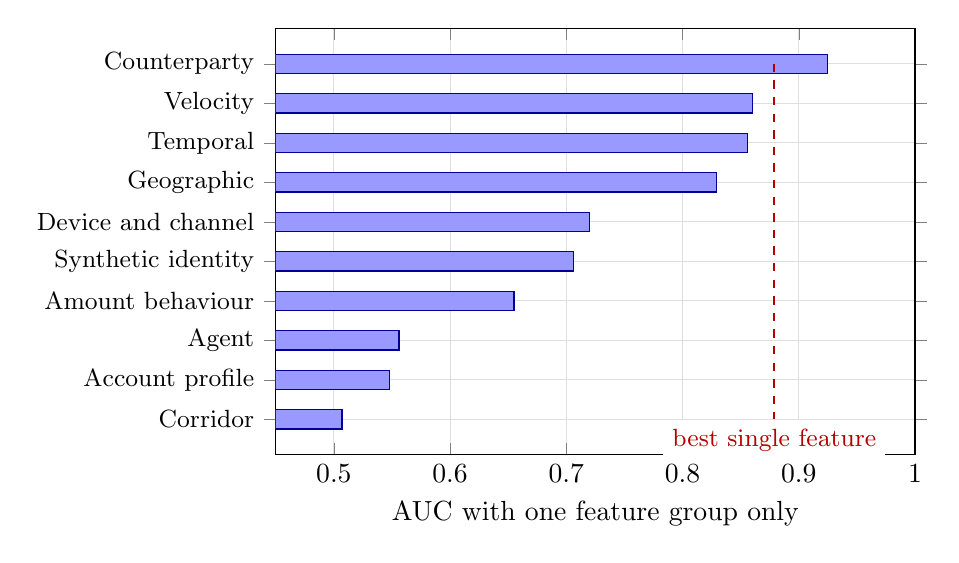
\begin{tikzpicture}
  \begin{axis}[
      width=0.8\linewidth, height=7cm,
      xbar, bar width=7pt, xmin=0.45, xmax=1.0,
      xlabel={AUC with one feature group only},
      symbolic y coords={{Counterparty},{Velocity},{Temporal},{Geographic},{Device and channel},{Synthetic identity},{Amount behaviour},{Agent},{Account profile},{Corridor}},
      ytick=data, y dir=reverse, yticklabel style={font=\small},
      grid=major, grid style={gray!25},
    ]
    \addplot[fill=blue!40, draw=blue!60!black] coordinates {(0.925,{Counterparty}) (0.86,{Velocity}) (0.856,{Temporal}) (0.829,{Geographic}) (0.72,{Device and channel}) (0.706,{Synthetic identity}) (0.655,{Amount behaviour}) (0.556,{Agent}) (0.548,{Account profile}) (0.507,{Corridor})};
    \draw[red!70!black, thick, dashed] (axis cs:0.879,{Counterparty}) -- (axis cs:0.879,{Corridor})
      node[pos=1, anchor=north, font=\small, fill=white] {best single feature};
  \end{axis}
\end{tikzpicture}

\caption{AUC of the diagnostic model with one feature group only (Table~\ref{tab:groups}), against the
best single feature on the same test rows (\nGateFloor{}, dashed). Four groups reach at least
\nGroupGeographic{} alone. Generated by \texttt{figures/make\_figures.py} from \texttt{numbers.tex}.}
\label{fig:groups}
\end{figure}

The benchmark can be solved several different ways, so no single group is load-bearing and a
leave-one-group-out ablation reports each as nearly free. This is a result about how a
scenario-driven generator encodes signal: a generator that plants fraud as incidents writes the
same structure into the velocity, counterparty, temporal and geographic views at once. On the
earlier draw \texttt{6abde44e} the same four groups each reached at least \nEarlyGroupMin{}; the
threshold moved with the draw and the finding did not.

It also disposes of a planned experiment. The specification's claim that models built elsewhere
reach far lower AUC on East African mobile money data is unverified (claims register, C-4), and
the proposed replacement, a card-style feature set against the full set, cannot answer it here:
the production ensemble restricted to card-style features changes AUC by \nAblCardD{}, and on a
benchmark this redundant a subset comparison shows a small difference whatever is true of real
systems. The specification's other ablations of the production ensemble are equally small
(without agent features \nAblAgentD{}, without the corridor feature \nAblCorridorD{}, without
round-sum awareness \nAblRoundD{}, without month-end awareness \nAblMonthD{}, without USSD-aware
device handling \nAblUSSDD{}) and are reported for completeness, not as evidence of what matters
in production.

\subsection{Calibration and explanation}

The row-weighted calibration error is nearly meaningless at a base rate below one per cent: almost every
row sits in the lowest bin, where no decision is made. On the diagnostic model we therefore also
report it in the decision region (score at or above the flag threshold, \nBatDecisionRows{} rows):
\nBatECEDecision{}, against \nBatECEAll{} over all rows. The additivity error of the exact TreeSHAP
contributions, which must sum to the model's margin, is \nBatAdditivity{}.

\subsection{The latency--explainability frontier}
\label{sec:frontier}

Resolution D-16 makes tree complexity a constrained hyperparameter: a configuration whose
single-request 99th-percentile latency, model plus exact TreeSHAP, exceeds 40~ms is rejected.
Table~\ref{tab:frontier} is the trade-off, measured one request at a time (a batch would amortise
exactly the overhead a single request pays), \nFrRequests{} timed requests per configuration after
a warm-up, on the development laptop.

\begin{table}[htbp]
\centering
\caption{Accuracy and median single-request latency across tree complexity (one XGBoost booster,
draw \texttt{6abde44e}, \nFrHeldOutRows{} held-out rows holding \nFrHeldOutFraud{} fraud,
\nFrRequests{} timed requests per configuration, evidence commit \texttt{95b722c}, source
\texttt{docs/benchmarks/m4\_frontier\_6abde44e.txt}). Milliseconds
are from the development laptop and are not gate figures (ADR 0010).}
\label{tab:frontier}
\begin{tabular}{rrrrrr}
\toprule
Trees & Depth & AUC & Predict p50 (ms) & With SHAP p50 (ms) & SHAP cost (ms) \\
\midrule
50 & 3 & \nFrAucA & \nFrPredA & \nFrShapA & \nFrCostA \\
100 & 4 & \nFrAucB & \nFrPredB & \nFrShapB & \nFrCostB \\
200 & 5 & \nFrAucC & \nFrPredC & \nFrShapC & \nFrCostC \\
400 & 6 & \nFrAucD & \nFrPredD & \nFrShapD & \nFrCostD \\
800 & 8 & \nFrAucE & \nFrPredE & \nFrShapE & \nFrCostE \\
\bottomrule
\end{tabular}
\end{table}

\begin{figure}[htbp]
\centering
% Generated by figures/make_figures.py from numbers.tex; do not edit.
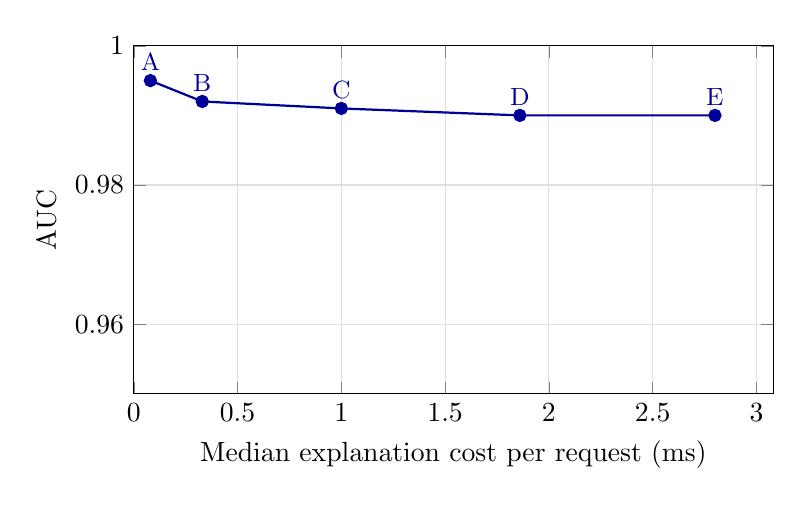
\begin{tikzpicture}
  \begin{axis}[
      width=0.8\linewidth, height=6cm,
      xlabel={Median explanation cost per request (ms)},
      ylabel={AUC}, ymin=0.95, ymax=1.0, xmin=0,
      grid=major, grid style={gray!25},
      nodes near coords, point meta=explicit symbolic,
      every node near coord/.append style={font=\small, anchor=south},
    ]
    \addplot[mark=*, thick, blue!60!black] coordinates {
      (0.08, 0.995) [A]
      (0.33, 0.992) [B]
      (1.0, 0.991) [C]
      (1.86, 0.99) [D]
      (2.8, 0.99) [E]
    };
  \end{axis}
\end{tikzpicture}

\caption{The frontier of Table~\ref{tab:frontier}: AUC against the median cost of an exact TreeSHAP
explanation, one point per configuration (A: the smallest, E: the largest). Accuracy stays within
its interval while the cost grows. Generated by \texttt{figures/make\_figures.py} from
\texttt{numbers.tex}.}
\label{fig:frontier}
\end{figure}

From the smallest configuration to the largest, AUC moves \nFrontAUCDelta{}, inside every
interval, while the median cost of explaining a decision grows about \nFrontRatio-fold, from
\nFrontShapSmall{} to \nFrontShapLarge{}~ms; prediction alone grows from \nFrontPredSmall{} to
\nFrontPredLarge{}~ms. The accuracy half is a property of this easy benchmark and should not be
generalised. The latency half is a property of the model and the explanation algorithm: exact
TreeSHAP costs $O(TLD^2)$ for $T$ trees with at most $L$ leaves and depth $D$
\cite{lundberg2020trees}, which is why an easy benchmark cannot weaken it.

Three cautions keep this result in proportion. First, every configuration explains a decision in a
few milliseconds at the median, far inside the specification's 40~ms per-request budget, so on this
evidence explanation cost binds at throughput (the work each core does per explained request)
rather than at the latency of a single request. Second, the \nFrontRatio-fold ratio depends on the
grid: it is measured from the cheapest configuration tried, and a different smallest configuration
would give a different ratio; the growth with trees and depth is the finding, not the number.
Third, it is one machine's median. On data like this, the explanation budget, not the accuracy
target, should choose the tree configuration.

\textbf{We report the median only.} In \nFrontNegative{} configurations the measured 99th
percentile shows a \emph{negative} explanation cost, which is impossible: explaining cannot be
faster than not explaining. The tail on this shared machine is scheduler jitter, not model
complexity. D-16's 40~ms constraint therefore cannot be applied from this run; the
99th-percentile frontier on a dedicated machine is \notyet{M10}. Three further limits: one model
family (not the ensemble), one process (not the specified multi-process service), and a SHAP cost
paid on every row, whereas in serving it is paid only on flagged transactions.

\subsection{What this evaluation does not yet report}

\begin{itemize}
  \item Precision at a fixed analyst alert budget, the operational number: \notyet{M4 follow-up}.
  \item Performance by month of the test period (claims register, C-5): \notyet{M4 follow-up}.
  \item The cost curve of fraud loss prevented against legitimate transactions blocked and
        reviews required: \notyet{M4 follow-up}.
  \item Leave-one-fraud-type-out and the value of Isolation Forest routing for novelty:
        \notyet{M4 follow-up}.
  \item Shadow-mode AUC delta and scoring latency of the serving path: \notyet{M5}.
  \item End-to-end decision latency and throughput at the specified load: \notyet{M6 and M10}.
\end{itemize}
